\documentclass[Lau,noexaminfo,oneside,binding=0.6cm]{sapthesis}
\usepackage[T1]{fontenc}
\usepackage[utf8]{inputenc}
\usepackage[italian]{babel}
\usepackage{lipsum}
\usepackage{url}
\usepackage{hyperref}
\usepackage{graphicx}
\usepackage{placeins}
\usepackage{listings}
\usepackage{array}
\usepackage{wrapfig}
\usepackage{hyperref}
\usepackage{multicol,caption}
\usepackage[bottom]{footmisc}


\definecolor{codegreen}{rgb}{0,0.6,0}
\definecolor{codegray}{rgb}{0.5,0.5,0.5}
\definecolor{codepurple}{rgb}{0.58,0,0.82}
\definecolor{backcolour}{rgb}{0.95,0.95,0.92}

 
\lstdefinestyle{mystyle}{
    backgroundcolor=\color{backcolour},   
    commentstyle=\color{codegreen},
    keywordstyle=\color{magenta},
    numberstyle=\tiny\color{codegray},
    stringstyle=\color{codepurple},
    basicstyle=\footnotesize,
    breakatwhitespace=false,         
    breaklines=true,                 
    captionpos=b,                    
    keepspaces=true,                 
    numbers=left,                    
    numbersep=5pt,                  
    showspaces=false,                
    showstringspaces=false,
    showtabs=false,                  
    tabsize=2
}
 
\lstset{style=mystyle}

\graphicspath{ {images/} }
\hypersetup{
    colorlinks,
    citecolor=black,
    filecolor=black,
    linkcolor=black,
    urlcolor=black
}

\courseorganizer{Sapienza Università di Roma }
\advisor{Prof. Andrea Vitaletti}
\course{Ingegneria Informatica}
\IDnumber{1649359}
\submitdate{2018/2019}
\copyyear{2019}
\authoremail{edo.puglisi95@gmail.com}
\author{Edoardo Puglisi}
\title{MoveMate - ride pooling da studenti per studenti}
\subtitle{Metodologia Agile per lo sviluppo di applicazioni}


\begin{document}

\frontmatter
\maketitle
\dedication{Alla mia famiglia e alla Compagnia dell'Anello} 

\begin{abstract}
Durante il corso "Reti di calcolatori", tenuto dal professore Andrea Vitaletti, è stato proposto agli studenti di partecipare ad un laboratorio tenuto da Google presso l'Università La Sapienza relativo allo sviluppo cloud e web di servizi, nel corso del quale sono stati trattati argomenti relativi alla metodologia di sviluppo Agile e allo sviluppo di una corretta User Interface e relativa User Experience. L’obbiettivo era quello di fornire ai partecipanti le conoscenze necessarie per dare vita ad un’applicazione (web o nativa) seguendo le linee guida presentate durante le varie giornate del workshop stesso. 
Nel dicembre del 2016 il team di cui facevo parte ha iniziato a sviluppare l’applicazione: MoveMate. L’idea era di creare una piattaforma che consentisse agli studenti universitari romani (e in seguito di tutta Italia) di mettersi in contatto tra di loro così che potessero condividere il tragitto (e relative spese) verso (e da) le sedi universitarie. 
Partendo dall’idea del prototipo, attraverso tre milestones, ad aprile 2017 abbiamo portato a termine il lavoro con il rilascio al pubblico della versione finale dell'applicazione.
\end{abstract}

\mainmatter

\begin{acknowledgments}
Vorrei ringraziare il prof. Andrea Vitaletti che mi ha consigliato e spronato a dare il massimo durante tutto il periodo di lavoro su questo progetto. Senza di Lei non avrei mai potuto partecipare a questa fantastica esperienza.
Ringrazio i miei colleghi, passati e presenti, con cui ho condiviso gioie e dolori dell'università.
Un ringraziamento particolare ai miei genitori per il sostegno e la pazienza.
Infine ringrazio i miei migliori amici, sempre pronti a festeggiare o consolarmi dopo ogni esame, e la mia amica Lucia per il suo prezioso aiuto.
\end{acknowledgments}

\tableofcontents

\chapter{Metodologia Agile}
Nell'ingegneria del software, la metodologia agile si riferisce a un insieme di metodi di sviluppo del software derivati dai principi del "Manifesto per lo sviluppo agile del software" pubblicato nel 2001. I metodi agili propongono un approccio focalizzato sull'obiettivo di consegnare software funzionante e di qualità al cliente  in tempi brevi e frequentemente.
La metodologia agile è alla base del progetto descritto in seguito e del lavoro svolto durante tutto il periodo di sviluppo.

\section{Introduzione}
Fra le pratiche promosse dai metodi agili ci sono lo sviluppo iterativo e incrementale, la pianificazione adattiva, il coinvolgimento diretto e continuo del cliente nel processo di sviluppo e la formazione di piccoli team di lavoro.
La maggior parte dei metodi cosiddetti agili sviluppa il software in finestre di tempo limitate chiamate iterazioni che, in genere, durano qualche settimana. Nel caso di questo workshop le iterazioni erano rappresentate da tre "milestones" in cui i team dovevano presentare il lavoro svolto fino a quel momento. Ogni iterazione è un piccolo progetto indipendente e contiene tutto ciò che è necessario per rilasciare un piccolo incremento nelle funzionalità del software: planificazione (planning), analisi dei requisiti, progettazione, implementazione, test e documentazione. Alla fine di ogni iterazione il team deve rivalutare le priorità del progetto.
I metodi agili preferiscono la comunicazione in tempo reale a quella scritta.
Il team agile è composto da tutte le persone necessarie per terminare il progetto e includono anche il cliente.
L'obiettivo è la piena soddisfazione del cliente e non solo l'adempimento di un contratto. Le metodologie agile, inoltre, possono consentire all'abbattimento dei costi e dei tempi di sviluppo aumentando la qualità del prodotto finale.

\section{Principi}
I principi su cui si basa una metodologia agile sono quattro:
\begin{itemize}
\item le relazioni e la comunicazione tra gli attori di un progetto sono più importanti degli strumenti utilizzati;
\item è più importante avere software funzionante che documentazione;
\item bisogna collaborare con i clienti poichè la collaborazione diretta offre risultati migliori dei rapporti puramente contrattuali;
\item bisogna accettare il cambiamento e il team deve essere pronto a modificare le priorità di lavoro.
\end{itemize}

\section{Pratiche utilizzate}
Le singole pratiche applicabili all'interno di una metodologia agile sono molteplici e dipendono dalle necessità e dall'approccio scelto. Ogni pratica ha pro e contro. Ad esempio, in Extreme Programming (uno dei tanti metodi esistenti), la mancanza assoluta di qualsiasi forma di progettazione e documentazione è compensata con lo strettissimo coinvolgimento del cliente nello sviluppo e con la programmazione in coppia.
Sono elencate ore le pratiche utilizzate nel corso del progetto.

\begin{itemize}
\item \textbf{Coinvolgimento del cliente - }Vi sono differenti gradi di coinvolgimento (come detto precedentemente per il caso di Extreme Programming). In questo caso specifico il cliente è stato ascoltato in più occasioni: per la convalida dell'idea e per i successivi test sull'esperienza d'uso.
\item \textbf{Cultura di Team - }Fondamentale nel seguire approcci agili è la collaborazione e l'approccio mentale e pratico del team di sviluppo stesso. Ci si orienta verso un modus operandi "di gruppo" che andrà a premiare (o viceversa) il gruppo unicamente sulla base del raggiungimento degli obiettivi di team previsti per quel dato intervallo temporale.
\item \textbf{Consegne frequenti - }Le consegne frequenti garantiscono di continuare il lavoro da un codice già scritto nella consegna precedente , di  offrire al cliente una parte di progetto distraendolo fino alla consegna finale, di effettuare test su porzioni di applicazione e ricevere feedback su eventuali nuove funzionalità da inserire o correggere.
Le iterazioni sono rappresentate dalle tre milestones del workshop.
\item \textbf{Progettazione e documentazione - }Pensare che le metodologie leggere eliminino la progettazione e la documentazione è un errore. Infatti è sempre buona norma garantire e non trascurare la parte di progettazione e documentazione. In questo caso sono stati disegnati i diagrammi UML delle classi e dei casi d'uso.
\end{itemize}
\chapter{Fase iniziale}
In questo capitolo verrà esposta la fase iniziale del progetto: come è nata l'idea e quali sono stati i primi passaggi per gettare una solida base di un'applicazione che potesse risultare valida.

\section{Idea}
Alla base del workshop vi era sostanzialmente una gara tra team di programmatori con lo scopo di premiare l'applicazione migliore secondo parametri quali la scalabilità e utilità per il grande pubblico.
Studiando varie idee per il nostro progetto, abbiamo cercato di trovare un punto comune tra tutti i membri. Il principale punto di congiunzione tra noi era il fatto di vivere a pieno la vita da universitari con relativi problemi e difficoltà. Per questo abbiamo provato ad elaborare una soluzione ad almeno uno dei vari problemi che ci affliggevano e, di conseguenza, affliggevano gli altri studenti di tutte le univiversità.
Primo tra tutti, a rendere faticosa la vita studentesca, è il ‘viaggio’ giornaliero per raggiungere le sedi: ogni mattina uno studente si alza e sà che dovrà correre più veloce del tram per non perderlo e arrivare in ritardo a lezione. La maggior parte degli studenti, infatti, ogni giorno intraprende una vera e propria odissea per raggiungere le università a causa del traffico, dei ritardi dei mezzi pubblici e di tutte le scomodità che un pendolare può conoscere.
Una volta individuato il problema, ci siamo messi a lavoro per trovare una soluzione basandoci sulle idee proposte dai competitors e adattandole poi alla figura dello studente medio: da qui il nostro motto “For students. By students”.
Sono stati presi in considerazione diversi approcci al problema fino a giungere alla conclusione che quello del ride pooling fosse il più appropriato, perché in grado di unire il taglio dei costi e il fattore social.
A differenza del più famoso car sharing in cui l'utente di fatto noleggia un' auto, il ride pooling consiste nella condivisione di un passaggio e dei relativi costi come benzina e/o parcheggio.
Il possesso di un mezzo privato, per quanto conveniente, comporta molteplici costi, dal carburante al mantenimento, passando per il parcheggio e l’assicurazione; la condivisione invece permette di ripartire una parte di questi tra più persone; portando all’ammortamento dei costi intrinsechi del tragitto e alla riduzione del numero delle macchine in circolazione. Tutto ciò attraverso la messa in contatto di studenti, così da favorire l’incontro tra le diverse realtà universitarie e magari fare nuove amicizie.

\section{Convalida dell'idea}
Al fine di concretizzare il nostro lavoro ed essere sicuri che il progetto avesse un effettivo valore per il suo bacino di utenti, avevamo bisogno di un riscontro con il futuro pubblico dell’applicazione. Per questo è stato sottoposto un sondaggio ad un gran numero di studenti delle principali università di Roma.
Il sondaggio non doveva essere complesso per evitare di avere risultati falsati dalle risposte randomiche di eventuali studenti frettolosi nel rispondere e sostanzialmente anche perchè i concetti cardine da rilevare erano pochi.
Oltre il 75\% ( Figura \ref{fig:graph1} ) dei partecipanti al sondaggio ha risposto positivamente alla domanda “Utilizzeresti il servizio MoveMate?”.
Alla domanda “Come useresti il servizio?” quasi il 50\% ( Figura \ref{fig:graph2} ) era interessato al fattore social della nostra applicazione così da poter conoscere altre persone.
A tal fine abbiamo aggiunto la possibilità di "condividere" anche il viaggio con mezzi pubblici.
L’interesse da parte degli studenti ci ha dato coraggio nel continuare il nostro progetto.

\begin{figure}[!h]
\begin{minipage}{\linewidth}
  \centering
    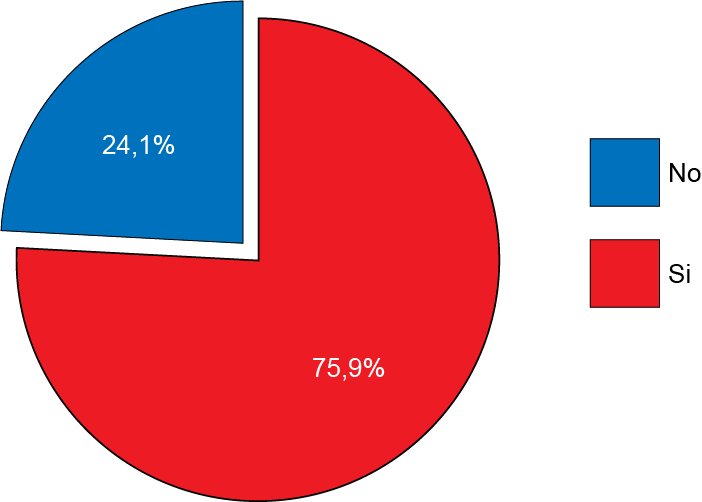
\includegraphics[width=0.6\textwidth]{graph1}
  \caption{Snapshot risultati 1}
  \label{fig:graph1}
\vspace{1cm}
  \centering
    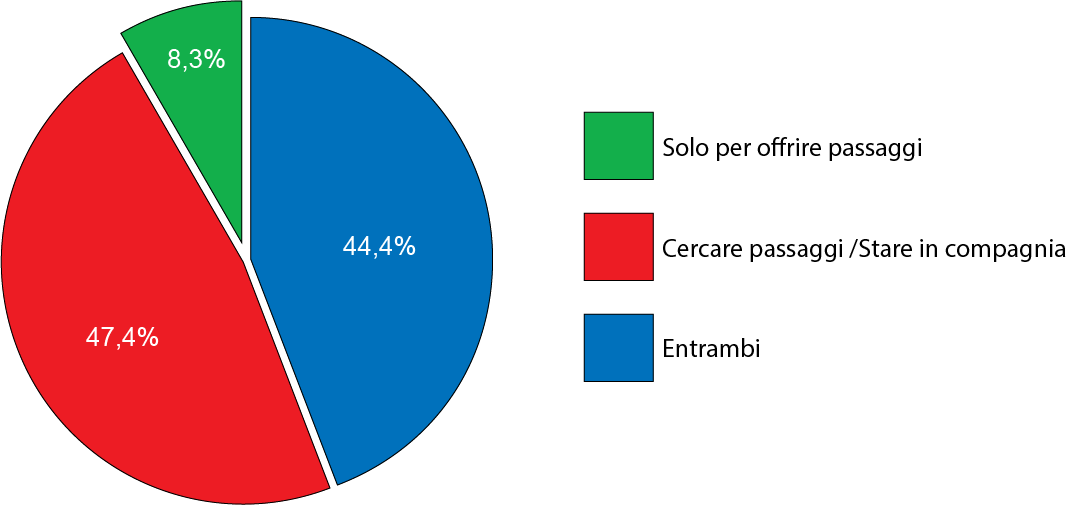
\includegraphics[width=0.9\textwidth]{graph2}
  \caption{Snapshot risultati 2}
  \label{fig:graph2}
\end{minipage}
\end{figure}

\FloatBarrier



\chapter{Progettazione}
Prima di passare alla parte di scrittura del codice si deve decidere "cosa" dovrà fare il codice e come sarà strutturata l'anima dell'applicazione.

\section{Preparazione}
Convalidata l’idea, sono state selezionate le “features” che l’applicazione avrebbe dovuto avere sulla base delle risposte ai sondaggi somministrati agli studenti dei principali atenei di Roma. Il target sarebbe stato un pubblico giovane con bisogni precisi e su di essi è stata costruita la struttura dell’applicazione, tenendo conto delle linee guida della programmazione AGILE, partendo dal modello UML.
Sono state scelte le tecnologie da utilizzare in funzione del tipo di servizio offerto: si è optato per una applicazione mobile Android abbinata ad un server gestito da Microsoft Azure.
Lo sviluppo del progetto è stato suddiviso tra i membri del team per competenze riguardanti i linguaggi di programmazione, tra lato client (Android) e lato server (ASP.Net) , in modo tale da velocizzare il lavoro annullando il tempo di apprendimento di una nuova tecnologia.
Il workshop ci ha fornito la possibilità di lavorare come una squadra per il raggiungimento di un obbiettivo comune e concreto, mettendoci nella condizione di procedere ad un buon ritmo di lavoro, ma soprattutto ci ha dato l’opportunità di iniziare un fondamentale accrescimento personale, fornendoci gli strumenti necessari, accademici e non, in vista di future attività lavorative grazie ad una vera e propria simulazione di progetto aziendale.

\section{Modello UML}
In ingegneria del software, UML (unified modeling language, "linguaggio di modellizzazione unificato") è un linguaggio di modellazione e specifica basato sul paradigma orientato agli oggetti. Il linguaggio nacque con l'intento di unificare approcci precedenti, raccogliendo le migliori prassi nel settore e definendo così uno standard industriale unificato.
UML svolge un'importantissima funzione di "lingua franca" nella comunità della progettazione e programmazione a oggetti. Gran parte della letteratura di settore usa UML per descrivere soluzioni analitiche e progettuali in modo sintetico e comprensibile a un vasto pubblico.
La notazione UML è semi-grafica e semi-formale; un modello UML è costituito da una collezione organizzata di diagrammi correlati, costruiti componendo elementi grafici ed elementi testuali.
Per questo progetto sono state utilizzate due implementazioni di tale linguaggio: il class diagram, necessario per esplicitare il rapporto tra i vari Models ovvero le classi che compongono l'applicazione, e l’ use case diagram, necessario per mostrare il “workflow” dell’interazione tra utente e applicazione.

\subsection{Diagramma delle classi}
Il diagramma delle classi è uno dei tipi di diagrammi del modello UML. Il suo scopo è di rendere visiva l’interazione tra le entità che popoleranno il programma finale. Le relazioni che connettono i modelli rappresentano i legami tra di essi e possono essere accompagnate da ulteriori informazioni, ruolo e molteplicità, per specificare al meglio i vari vincoli.
Ad esempio, nel caso specifico, le due connessioni che collegano il modello Studente con il modello Path mostrano come uno studente possa far parte di molteplici “percorsi” e esserne creatore di altrettanti, ma un percorso può avere un solo creatore. 
La figura  \ref{fig:uml} mostra il digramma completo.

\subsection{Diagramma dei casi d'uso}
Il diagramma dei casi d’uso si occupa invece della descrizione delle funzioni del sistema dal punto di vista degli attori che interagiscono con esso. Questo tipo di diagramma può essere considerato come uno strumento per la rappresentazione dei requisiti funzionali del sistema poiché evidenzia le operazioni che l’utente (Studente) può effettuare (Figura \ref{fig:use-case}).
I "casi" di questo diagramma verranno poi implementati come funzioni che l'applicazione dovrà eseguire.
Le linee in grassetto indicano le operazioni base che l'utente puo compiere.
Tra le varie operazioni possono esistere delle relazioni: <include> indica che l'operazione alla base della freccia è eseguita dopo (o in contemporanea) l'operazione che si trova all'altro capo, mentre <extend> indica che l'operazione alla base della freccia aggiunge funzionalità all'operazione verso cui punta la freccia stessa.
Come possiamo notare, infatti, tutte le operazioni richiedono che l'utente effettui la procedura di login prima di essere eseguite (<include>) mentre l'operazione di "join" aggiunge una funzionalità alla ricerca di un percorso (<extend>).

\begin{figure}[!hb]
  \centering
    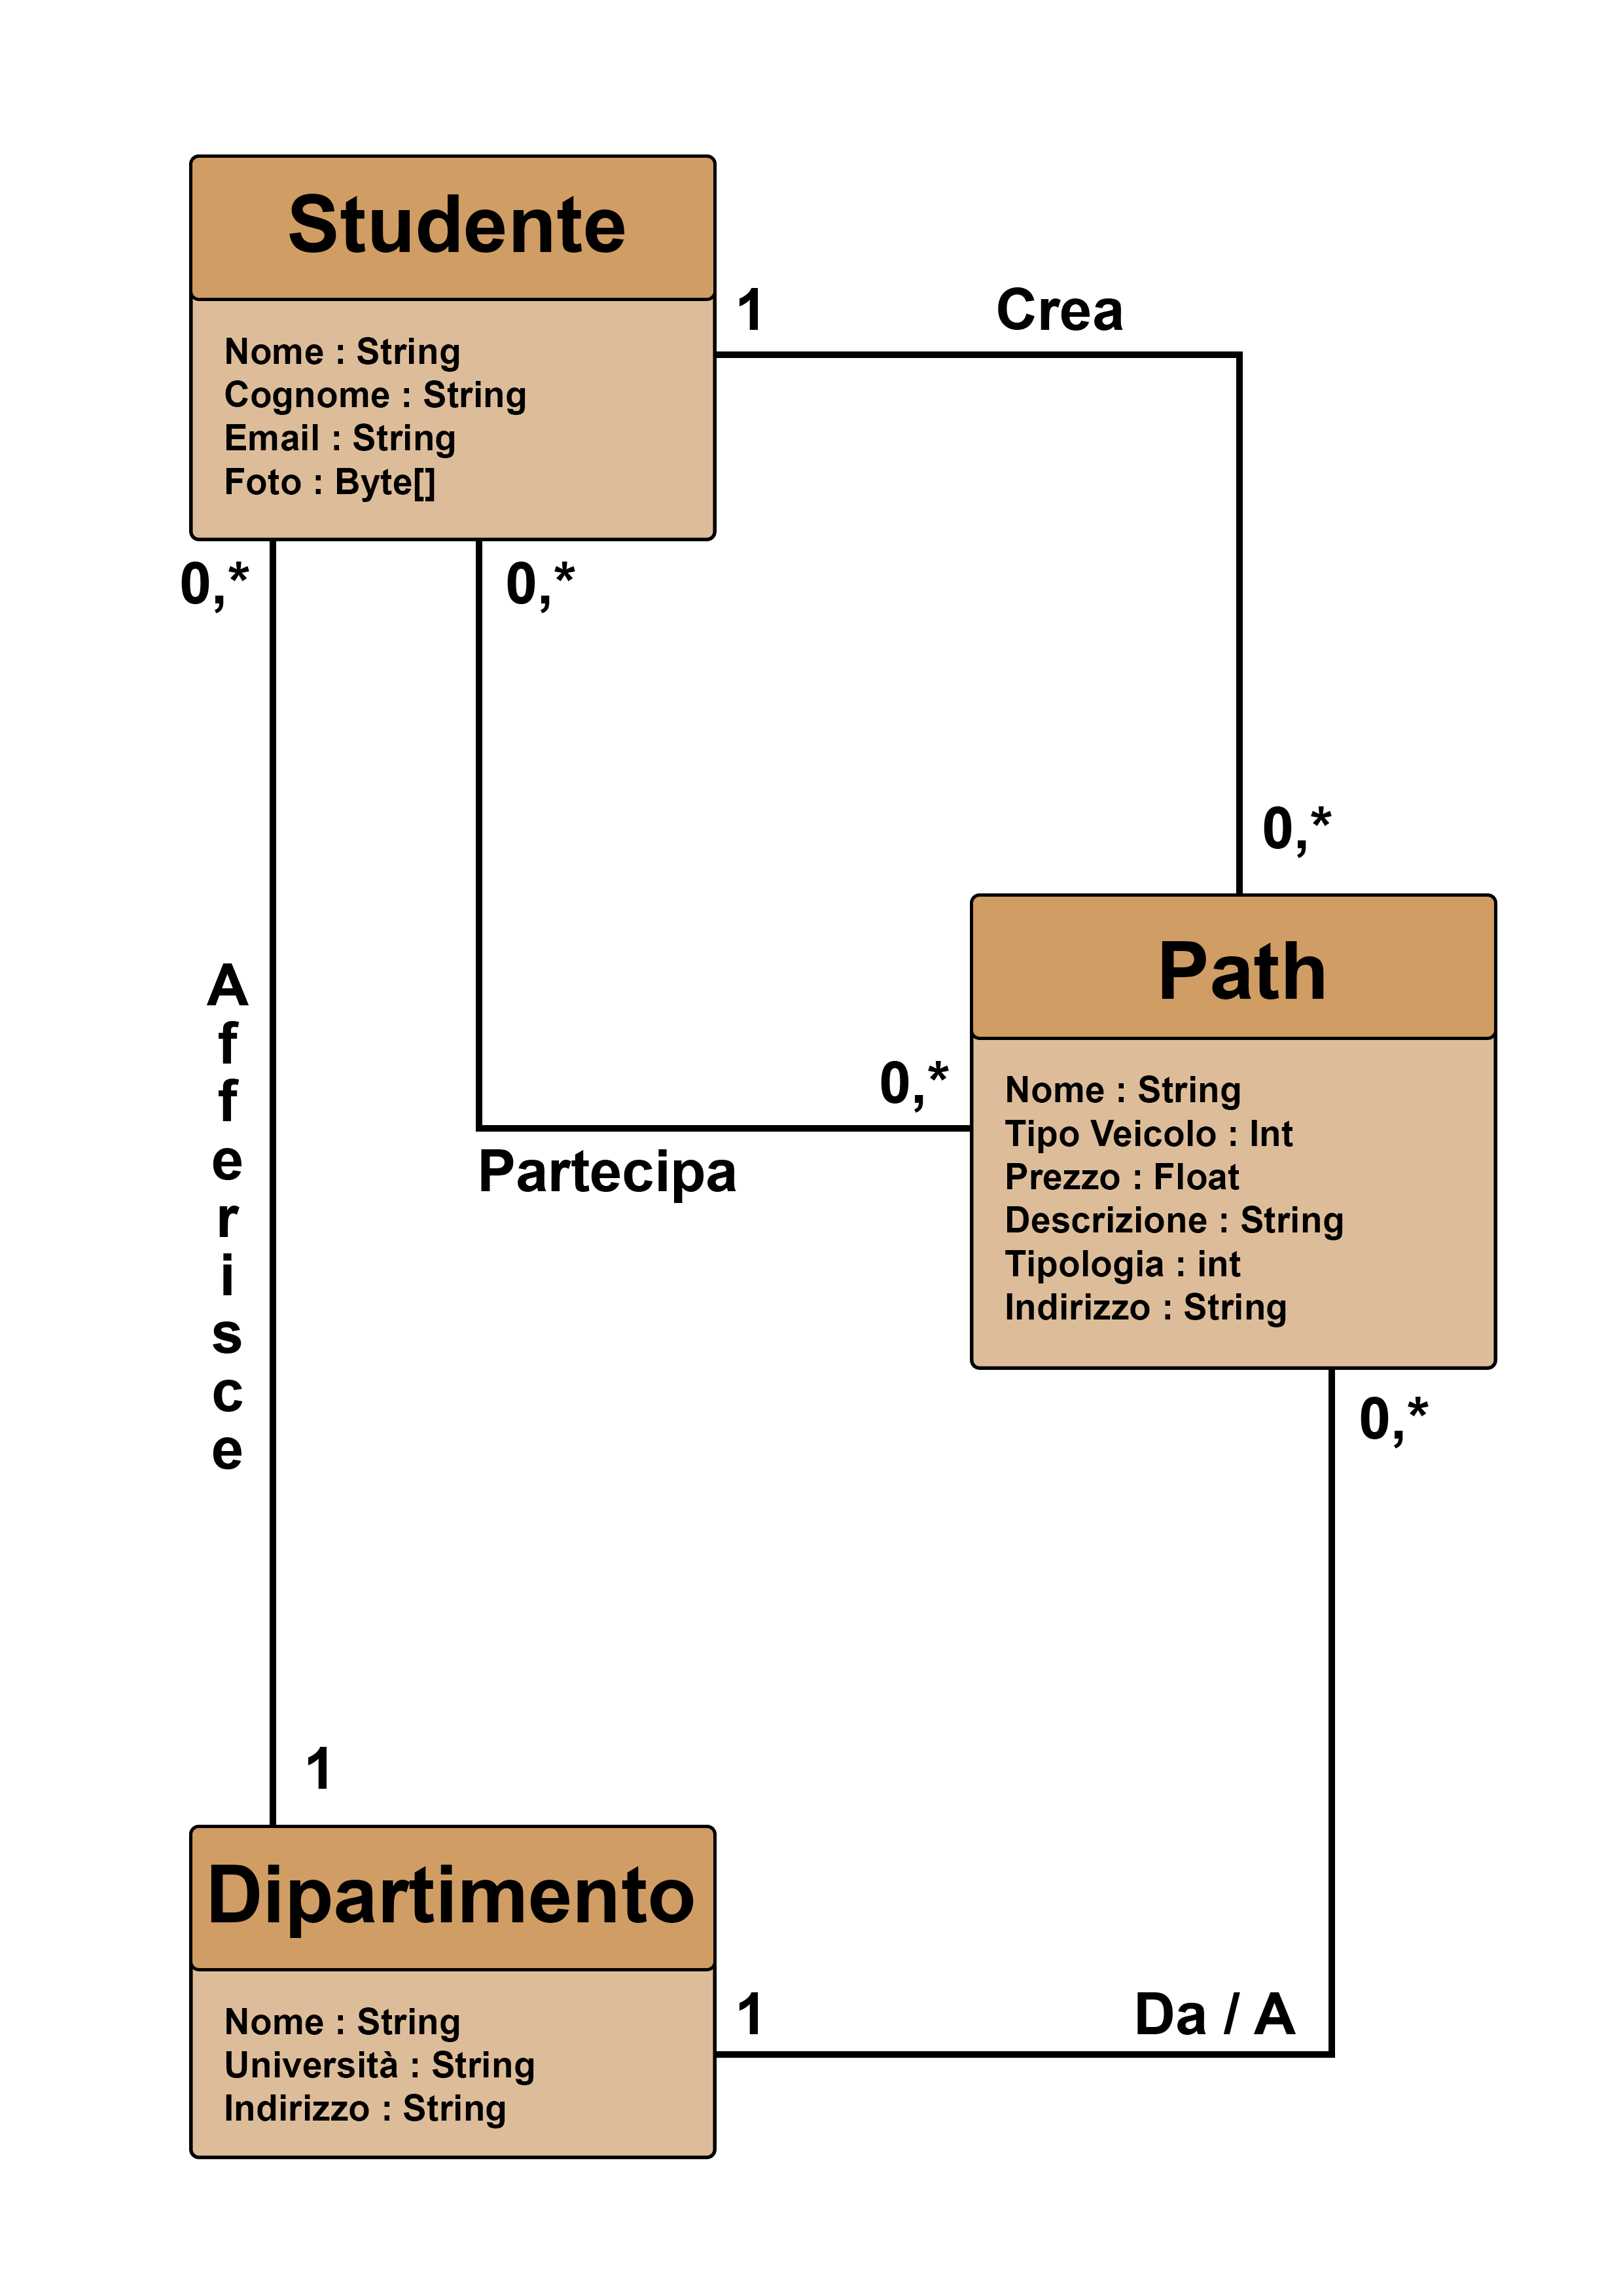
\includegraphics[width=1\textwidth]{uml}
  \caption{Diagramma delle classi}
  \label{fig:uml}
\end{figure}

\begin{figure}[!hb]
  \centering
    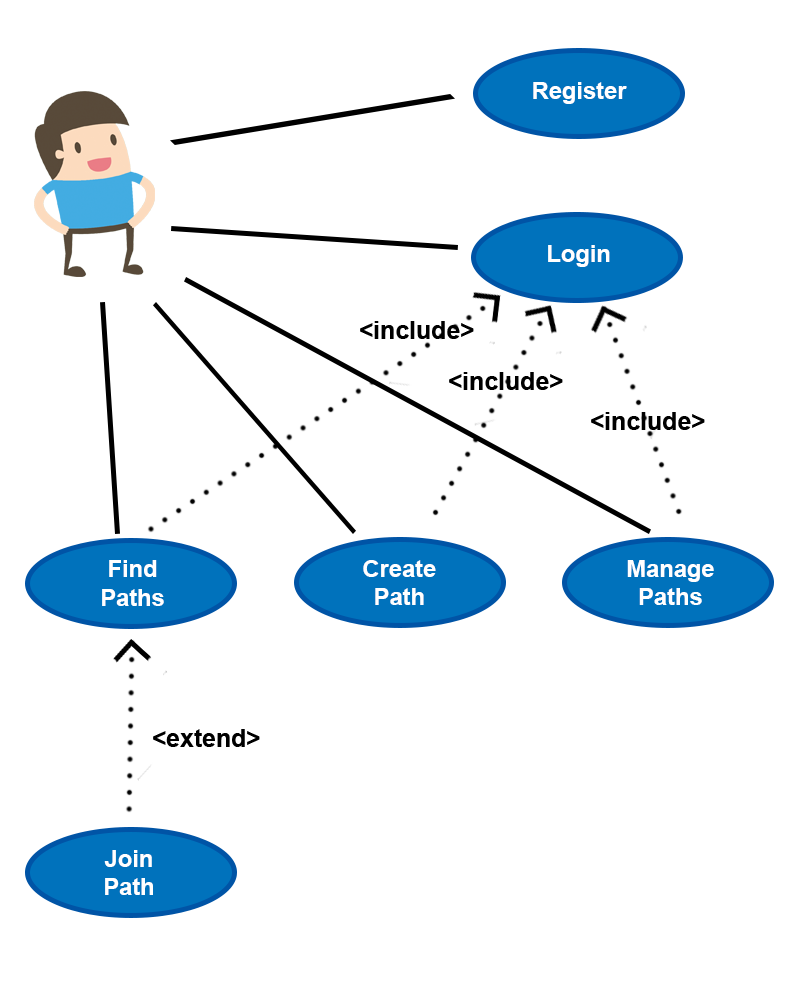
\includegraphics[width=1\textwidth]{use-case}
  \caption{Diagramma dei casi d'uso}
  \label{fig:use-case}
\end{figure}
\chapter{Tecnologie utilizzate}
Sono elencate ora le principali tecnologie utilizzate nel progetto. Alcune di esse avranno un ruolo prioritario in capitoli specifici.

\section{Android}
\begin{wrapfigure}{r}{0.1\textwidth}

\includegraphics[width=0.1\textwidth]{android-logo}
\end{wrapfigure} 
\FloatBarrier
Come vedremo nel capitolo ad esso dedicato, Android è più di un semplice linguaggio. Esso è infatti un ecosistema che unisce linguaggi di programmazione differenti con un sistema operativo sviluppato prettamente per dispositivi portatili.
Android nel caso specifico di questo progetto è l'ambiente di sviluppo utilizzato per dare vita al client.

\section{ASP.Net}
\begin{wrapfigure}{r}{0.2\textwidth}

\includegraphics[width=0.2\textwidth]{asp-logo}
\end{wrapfigure} 
\FloatBarrier
Sulle tecnologie ASP.Net si basa l' "anima" dell'applicazione: il server.
ASP.Net non è semplicemente un linguaggio di programmazione, ma un insieme di tecnologie di sviluppo software per il web commercializzate da Microsoft.
Come tutte le applicazioni della famiglia Microsoft.NET si basa sul Common Language Runtime (CLR): ovvero gli sviluppatori possono scrivere codice in uno dei qualsiasi linguaggi supportati (Visual Basic .Net, C\#, J\#, Python e molti altri) che verrà poi interpretato automaticamente.
Nello specifico è stato utilizzato il pattern Model-View-Controller (MVC) che approfondiremo nel paragrafo relativo al server.

\section{HttpS}
\begin{wrapfigure}{r}{0.2\textwidth}

\includegraphics[width=0.2\textwidth]{https-logo}
\end{wrapfigure} 
\FloatBarrier
L' HyperText Transfer Protocol (protocollo di trasferimento di un ipertesto) è , appunto, un protocollo usato come principale sistema per la trasmissione d'informazioni sul web e quindi su architetture client-server.
La "S" identifica la connessione criptata dal Transport Layer Security (TLS) o dal suo predecessore Secure Sockets Layer (SSL) che ne garantisce l'integrità.
Https lavora al livello più alto del modello TCP\footnote{Transmission Control Protocolo (TCP), protocollo a livello di rete che  rende affidabile la comunicazione dati tra mittente e destinatario.}/IP, il livello di applicazione. In pratica, tra il protocollo TCP e Http si interpone un livello di crittografia/autenticazione che cripta il messaggio Http prima della trasmissione e lo decripta una volta arrivato a destinazione. In pratica viene stabilita una connessione criptata tra client e server tramite lo scambio di certificati che attestano l'identità delle due controparti.

\section{OAuth}
\begin{wrapfigure}{r}{0.2\textwidth}

\includegraphics[width=0.2\textwidth]{oauth-logo}
\end{wrapfigure} 
\FloatBarrier
OAuth è un protocollo che permette l'autorizzazione di API\footnote{Con Application Programming Interface (API) si indica ogni insieme di procedure disponibili al programmatore, di solito raggruppate a formare un set di strumenti specifici per l'espletamento di un determinato compito all'interno di un certo programma. Spesso con tale termine si intendono le librerie software disponibili in un certo linguaggio di programmazione.} di sicurezza con un metodo standardizzato e semplice per ogni tipo di applicazione, sia esso mobile o fisso. Questo sistema permette ai service providers, ovvero i fornitori di servizi che fanno uso di questo protocollo, di condividere informazioni specifiche dei propri utenti con servizi terzi proteggendone le credenziali (per esempio la password).
Per capirne il funzionamento prendiamo come esempio il caso di login ad un qualsiasi sito web tramite account Facebook:
\begin{enumerate}
\item L'utente accede al sito e avvia la procedura di login tramite Facebook
\item L'utente inserisce le sue credenziali per garantire l'accesso alle sue informazioni
\item Il service provider (Facebook) risponde con un Access Token univoco
\item Il sito web utilizzerà l'Access Token per accedere alle informazioni dell'utente senza saperne le credenziali
\end{enumerate}
\chapter{Android}
Facciamo una panoramica su cosa è realmente Android.
Android non è un linguaggio di programmazione, ma un vero e proprio insieme di strumenti e librerie per la realizzazioni di applicazioni mobili.Un aspetto fondamentale del successo di Android è stato il fatto che il linguaggio da esso utilizzato si tratta del ben noto Java. Per rendere, però, eseguibile il codice Java su dispositivi mobili e quindi con risorse hardware limitate sono stati adottati accorgimenti, architetturali e software, per sfruttare al massimo le risorse disponibili.
Il principale cambiamento è stato l'adozione di una nuova Virtual Machine (VM) ottimizzata per l'esecuzione di applicazioni in ambienti a memoria ridotta: la Delvik Virtual Machine (DVM) adottata, infatti, è in grado di eseguire codice contenuto all'interno di file con estensione .dex ottenuti a partire dal byte-code Java con una riduzione di spazio del 50\% . Il Garbage Collector ovvero quella modalità automatica di gestione della memoria che libera le porzioni di memoria non utilizzate è rimasto invariato per non dover lasciare questo compito agli sviluppatori e alleggerirne il lavoro.

\section{L'architettura di Android}
Android ha un'architettura a layer, dove i livelli inferiori offrono servizi ai livelli superiori, che comprende l'insieme degli strumenti per la creazione delle applicazioni per dispositivi mobili, tra cui un sistema operativo, librerie native e Java e una VM dedicata (Figura \ref{fig:architettura-android}).

\begin{figure}[!ht]
  \centering
    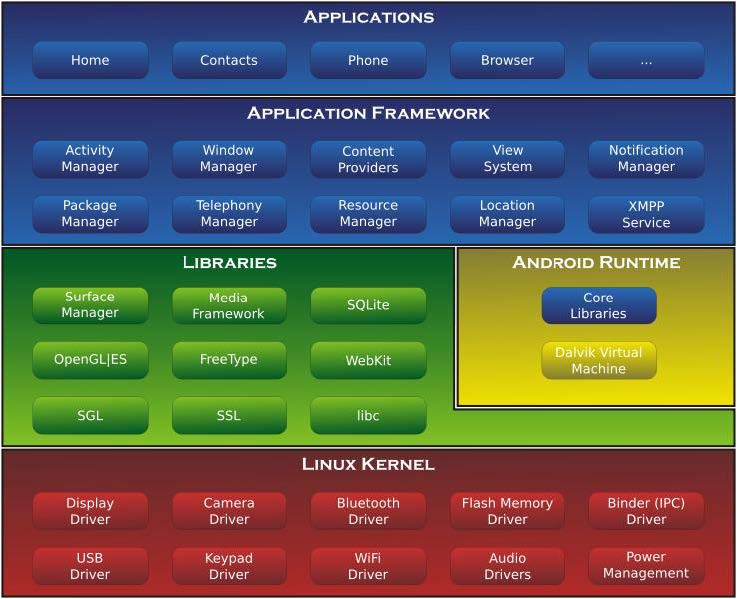
\includegraphics[width=1\textwidth]{architettura-android}
  \caption{Layers architettura Android}
  \label{fig:architettura-android}
\end{figure}
\FloatBarrier
Vediamo ora le sue componenti.

\subsection{Il kernel Linux}
Il livello più basso (in rosso) è occupato dal kernel\footnote{Il kernel costituisce il nucleo di un sistema operativo. Si tratta di un software avente il compito di fornire ai processi in esecuzione sull'elaboratore un accesso sicuro e controllato all'hardware. Dato che possono esserne eseguiti simultaneamente più di uno, il kernel ha anche la responsabilità di assegnare una porzione di scheduling e di accesso all'hardware a ciascun programma (multitasking).} Linux la cui presenza si è ritenuta necessaria per disporre di un vero e proprio sistema operativo che fornisse gli strumenti di basso livello per la virtualizzazione dell'hardware sottostante attraverso driver per la gestione di periferiche di ogni tipo.

\subsection{Librerie native}
Il livello seguente (in verde) è composto da un insieme di librerie standard redatte in C/C++ che rappresentano il core vero e proprio di Android.
\begin{itemize}
\item \textbf{Surface Manager (SM):}  ha il compito di gestire le View (come vedremo in seguito nel capitolo relativo al server) controllando e gestendo le diverse finestre visibili su schermo evitandone, per esempio, la sovrapposizione.
\item \textbf{OpenGL ES:} avendo risorse limitate c'è bisogno di applicare dei cambiamenti anche sul lato della grafica (2D e 3D) e per questo motivo è stato inserito un sottoinsieme delle API dell'OpenGL per semplificare e ottimizzare l'esecuzione delle operazioni di calcolo e rendering.
\item \textbf{SGL:} motore grafico per livelli 2D.
\item \textbf{Media Framework:} contiene le librerie per riprodurre i principali formati audio e video.
\item \textbf{WebKit:} browser-engine che viene integrato in diversi tipi di applicazioni.
\item \textbf{SSL:} librerie per gestire tutti i problemi legati alla sicurezza.
\item \textbf{SQLite:} un potente, ma leggero engine per database relazionali disponibile per tutte le applicazioni.
\item \textbf{FreeType:} librerie per bitmap e vettoriali per font.
\item \textbf{libc:} come si può intuire dal nome, è un'implementazione di librerie C standard, modificate per dispositivi basati su Linux.
\end{itemize}

\subsection{Android Runtime}
È il punto di distinzione tra un sistema operativo Android e un implementazione Linux per dispositivi mobili. È compoto dalla DVM e dalle librerie core che includono gran parte delle funzioni delle librerie standard di Java e ulteriori librerie specifiche per Android. Si occupa della gestione della memoria, della connettività e dei driver necessari al funzionamento di tutto l'ecosistema.

\subsection{Application Framework}
Fornisce i servizi di alto livello alle applicazioni sottoforma di classi Java. Gli sviluppatori sono liberi di utilizzare questi servizi nelle proprie applicazioni.
\begin{itemize}
\item \textbf{Activity Manager:} gestisce il ciclo vitale delle activity nelle applicazioni. Un activity è alla base di qualunque applicazione Android e sostanzialmente consiste nella finestra in cui verrà visualizzata l'interfaccia grafica.
\item \textbf{Content Providers:} gestisce lo scambio di dati tra un'applicazione e l'altra.
\item \textbf{Telephony Manager:} si occupa di tutte le chiamate vocali. Se un applicazione ha necessità di accedere alle chiamate dovrà utilizzare questa componente.
\item \textbf{Location Manager:} fornisce la geolocalizzazione grazie a GPS e ripetitori.
\item \textbf{Resource Manager:} tutti i tipi di risorse di cui un applicazione ha bisogno sono controllate da questo programma.
\item \textbf{Windows Manager:} gestisce le finestre delle diverse applicazioni attive sul dispositivo e relativa visualizzazione.
\item \textbf{Package Manager (PM):} permette alle applicazione di accedere a dati condivisi.
\item \textbf{View System:} fornisce gli strumenti per gestire gli elementi grafici ed arricchirli. Una TextView è per esempio un astrazione della semplice stringa.
\item \textbf{Notification Manager:} permette alle applicazioni di interagire con l'utente tramite notifiche.
\end{itemize}

\subsection{Applications}
L'ultimo livello è occupato dalle applicazioni installate nel sistema, siano esse native o di terze parti. Android non fa differenza tra applicazioni native e quelle provenienti da altre fonti garantendo ad entrambe gli stessi privilegi.

\section{Activity}

\begin{wrapfigure}{r}{0.4\textwidth}
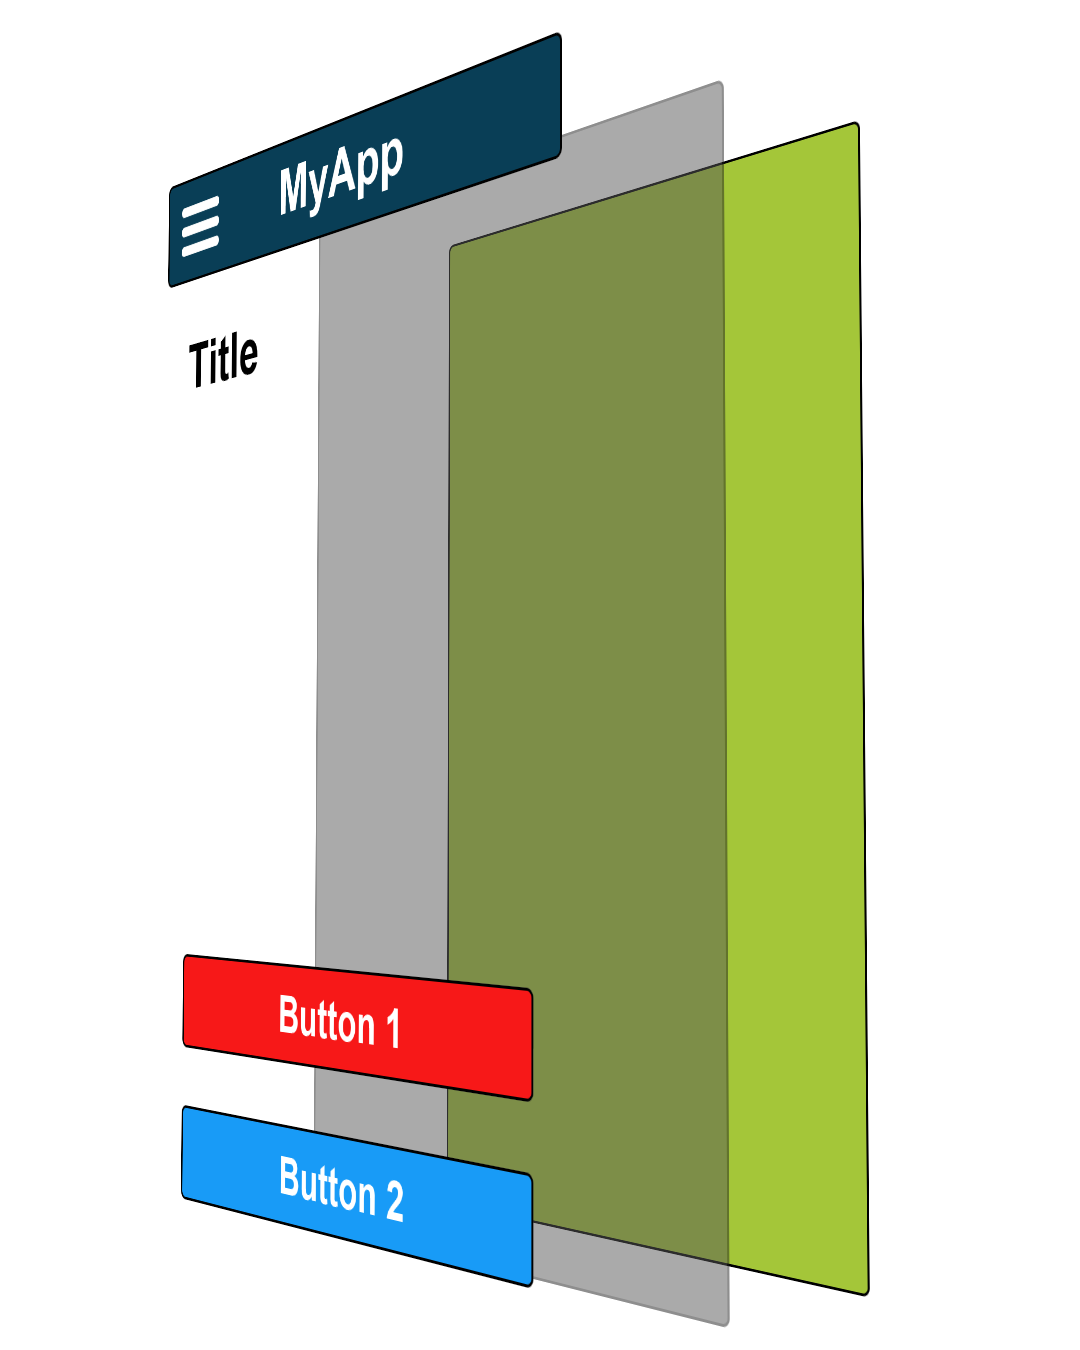
\includegraphics[width=0.4\textwidth]{activity}
\caption{View in Android}
\label{fig:activity}
\end{wrapfigure} 
\FloatBarrier

Parleremo nel capitolo seguente del paradigma MVC durante la descrizione del server, ma anticipiamo ora la sua descrizione lato client.
Sul client ci occuperemo solo della View (che scopriremo poi essere la parte interattiva di un sistema MVC).
Possiamo vedere il client come una sorta di telecomando che impartisce ordini al computer remoto che è il server.
La View di Android è chiamata Activity ed è alla base di ogni applicazione.
L'activity si occupa di creare la finestra nella quale lo sviluppatore inserirà il codice per l'interfaccia utente e di interpretare le azioni dell'utente in comandi da eseguire.
Da Android 3.0 si è aggiunta un'altra entità a sostegno dell'activity: il Fragment. I fragments sono una sorta di classe figlia della classe Activity e ne condividono gran parte del ciclo vitale (non può esistere un Fragment senza la sua activity). Essendo più "leggeri" di un activity a livello computazionale, più fragments possono coesistere sulla stessa activity contemporaneamente o sostituirsi tra loro.
In sostanza un'applicazione è composta come in Figura \ref{fig:activity}: in verde è rappresentata l'activity principale (un'applicazione può comunque passare da un'activity ad un altra a seconda dei casi) che gestirà le funzioni basilari dell'applicazione; sopra l'activity troviamo il fragment (in grigio): ogni fragment è una componente a sè stante che possiede le sue funzioni e relativo layout.
L'ultimo strato è appunto occupato dal Layout, ovvero la parte visibile ad occhio nudo, scritto in linguaggio XML associato a classi CSS.
\chapter{Sviluppo}
Vengono ora esposte le due "facce" del progetto: il back-end ed il front-end. In particolare ci si soffermerà sul lato client poichè fulcro dell'esperienza finale dell'applicazione.

\section{Architettura Server}
Questo paragrafo ha lo scopo di illustrare la composizione del server che gestisce tutte le funzioni "nascoste" del servizio e il suo funzionamento. A seguire una panoramica generale della sua architettura.

\begin{figure}[!h]
  \centering
    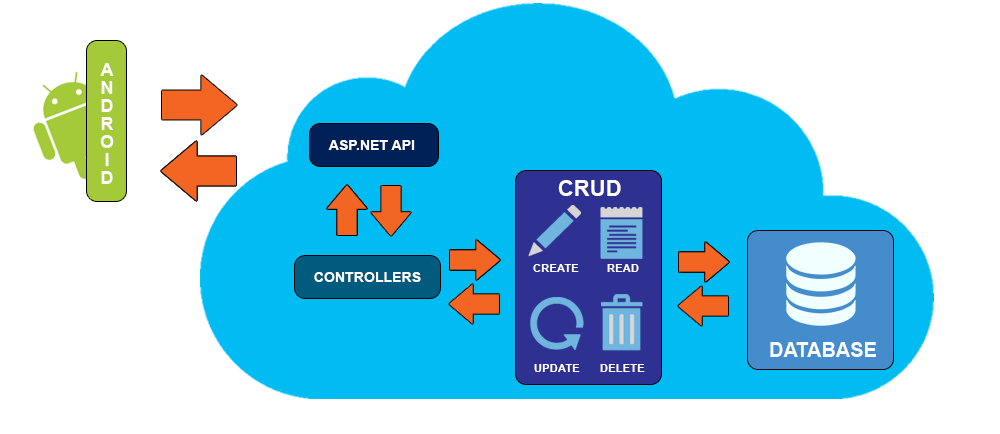
\includegraphics[width=1\textwidth]{server}
  \caption{Architettura server}
  \label{fig:server}
\end{figure}
\FloatBarrier

Il server è basato sulla piattaforma Microsoft Azure, programmato con tecnologia ASP.Net secondo il paradigma MVC (Model-View-Controller). MVC è un pattern architetturale molto diffuso nello sviluppo di sistemi software, in particolare nell'ambito della programmazione orientata agli oggetti, in grado di separare la logica di presentazione dei dati dalla logica di business.
\begin{itemize}
\item \textbf{Model:} rappresentano lo stato dell’applicazione, si occupano della gestione dei dati nel database e contengono i metodi per accedervi. Modifica, lettura e scrittura dei dati sono effettuate secondo il paradigma CRUD. I “risultati” sono inviati tramite View.
\item \textbf{View:} sono responsabili della presentazione dei dati richiesti tramite l’interfaccia utente ed è tramite esse che l’utente invia i comandi ai controllers. Nelle visualizzazioni la quantità di logica è minima e riservata alla presentazione del contenuto. Una view può essere una qualsiasi rappresentazione in output di informazioni, da un semplice grafico alla pagina web di un sito internet.
Come anticipato la View in Android è rappresentata dall'activity.
\item \textbf{Controller:} sono i componenti che gestiscono l’interazione tra l’utente e il Model e selezionano la corretta View da presentare come risultato finale. Nello schema MVC il controller è il punto di partenza poiché seleziona il Model (e relativa View) con cui interagire.
\end{itemize}
È possibile comprendere il funzionamento del paradigma MVC seguendo la semplice creazione di un “percorso” all’interno dell’applicazione.
\begin{enumerate}
\item Tramite l’UI (View) l’utente inizia la creazione del percorso: attraverso la procedura guidata inserisce in un pacchetto JSON tutte le informazioni utili (punto di partenza e arrivo, mezzo utilizzato, prezzo ecc).
\item Completata la procedura di acquisizione informazioni, la View invia i dati al Controller che si occupa della creazione del percorso tramite chiamata https (verso Google).
\item Il controller crea una nuova entità del Model “percorso” con le informazioni inserite dall’utente. Il Model si occuperà dell’inserimento del nuovo percorso nel database.
\item Il Controller aggiorna la View.
\item La View viene aggiornata e l’utente potrà visualizzare il nuovo percorso nell’homepage dell’applicazione.
\end{enumerate}

\section{Contributo personale}
Il mio compito all’interno del team riguardava lo sviluppo dell'interfaccia del progetto destinata all'utente finale. 
Le funzioni a cui mi sono dedicato possono riassumersi nelle seguenti categorie:
\begin{itemize}
\item \textbf{Login e autenticazione:} le operazioni che permettono all’utente di iniziare la propria esperienza d’uso all’interno dell’applicazione, identificandosi con il server e garantendone la sicurezza dei dati forniti tramite il protocollo OAuth. 
\item \textbf{Richieste HTTPS:} la gestione delle richieste verso il server e le risposte da esso con relativi dati allegati. Pertanto è stato necessario studiare e approfondire le meccaniche di funzionamento di una chiamata di REST nell'ecosistema Android.
\item \textbf{User Interface e User Experience:} l’interazione tra client e server tramite comandi grafici e la visualizzazione dei dati ricevuti in risposta (User Interface - UI); il tutto seguendo le linee guida necessarie ad una corretta User eXperience (UX) per mettere a proprio agio l’utente. A tal fine sono state prese in considerazione le risposte degli utenti ai nostri sondaggi.
\end{itemize}
Queste e altre funzioni verranno descritte nel dettaglio nelle sezioni successive.

\section{Architettura Client}
Come detto in precedenza il mio lavoro si è basato principalmente sullo sviluppo del client del nostro servizio ovvero l'applicazione Android con tutti i meccanismi che la compongono.
Di seguito è mostrata una panoramica della sua architettura:

\begin{figure}[!h]
  \centering
    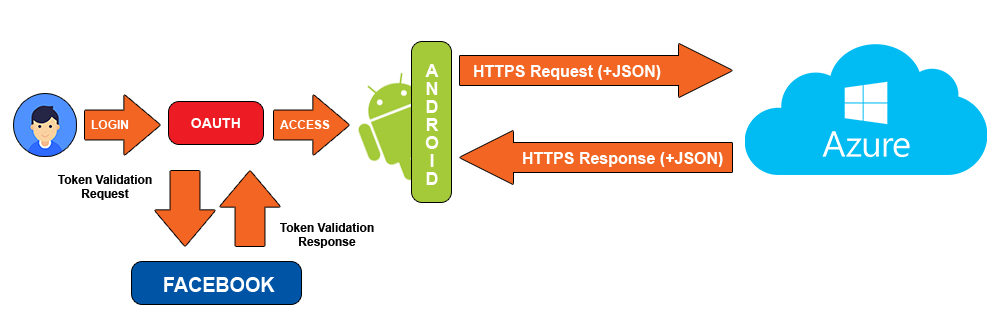
\includegraphics[width=1\textwidth]{client}
  \caption{Architettura client}
  \label{fig:client}
\end{figure}
\FloatBarrier

Il compito del client è di permettere all'utente di compiere operazioni inerenti al servizio a cui è collegato senza che esso sappia come esse vengano eseguite sul server.
L'utente (lo studente in questo caso) si limiterà ad effettuare il login, cercare (o creare) un passaggio e con un "click" potrà prenderne parte.
Vengono ora riportate le funzioni principali sulle quali si è basato il mio lavoro.

\subsection{Autenticazione OAuth}

\begin{wrapfigure}{r}{0.3\textwidth}

\includegraphics[width=0.3\textwidth]{login-button}
\caption{Sezione schermata login}
\label{fig:login-button}
\end{wrapfigure} 
\FloatBarrier

La prima schermata che l'utente incontrerà sarà quella di login.
È stato necessario trovare un metodo di login sicuro, che rientrasse nei parametri “user-friendly” ovvero gradevole alla vista e di facile utilizzo e che permettesse di identificare automaticamente molte informazioni dell’utente per velocizzare la procedura di registrazione. Tra le molteplici soluzioni possibili si è optato per l’accesso con protocollo OAuth tramite API Facebook.
OAuth è un protocollo aperto che permette ad un service provider (in questo caso Facebook) di condividere le informazioni personali di un utente con un consumer (in questo caso MoveMate) senza cedere le credenziali personali, il tutto ovviamente con il consenso dell'utente. È stato scelto questo metodo per poter unire la diffusione e facilità di utilizzo del servizio Facebook e la sicurezza del protocollo OAuth.
Alla pressione del pulsante di login (Figura \ref{fig:login-button}) inizierà il processo di autenticazione. Il tutto è gestito da una chiamata asincrona verso il server Facebook contenente un token di identificazione che verrà confermato lato server. Come mostrato nel listato \ref{lst:callback} la chiamata gestisce tre casi:

\begin{itemize}
\item \textbf{onSuccess:} rappresenta il caso di successo dell'autenticazione. Verrà chiamata la funzione interna check() detta callback\footnote{In programmazione, una callback è, in genere, una funzione, o un "blocco di codice" che viene passata come parametro ad un'altra funzione.} per il controllo dei dati utenti, in grado di verificare se si tratta di un utente già registrato o meno.
\item \textbf{onCancel:} è il caso in cui l'utente cancella la procedura di autenticazione prima del suo completamento. Nel nostro caso non verrà eseguita nessuna funzione e l'utente rimarrà nella schermata di login.
\item \textbf{onError:} indica il caso in cui sopraggiunga un errore di qualunque tipo e verrà mostrato il messaggio di errore a schermo.
\end{itemize}

In seguito al primo login (quindi nella funzione check()) è stato inserito un wizard\footnote{Nel linguaggio dell'informatica, il wizard (o autocomposizione) indica una procedura informatica, generalmente inglobata in una applicazione più complessa, che permette all'utente di eseguire determinate operazioni (solitamente complesse) tramite una serie di passi successivi.} che guida l’utente nella procedura di associazione tra il proprio profilo Facebook, le proprie credenziali universitarie (ateneo, matricola, email) e numero di telefono necessario per essere contattato dagli altri utenti.
Per la verifica dello status di studente e quindi garantire la partecipazione alla nostra community ai soli studenti, è stato implementato un sistema di verifica della casella di posta elettronica universitaria tramite invio e verifica di un codice univoco. Una volta terminata la procedura di identificazione iniziale, l’utente sarà in grado di accedere all’applicazione in maniera automatica grazie alle API Facebook e all’associazione ID Facebook – Email Studente.
Da questo momento in poi l'applicazione (precisamente il server) avrà tutti i dati dell'utente necessari al funzionamento del servizio.

\bigskip
\begin{minipage}{\linewidth}
\begin{lstlisting}[language=Java, caption=Esempio Facebook callback, label={lst:callback}]
FacebookSdk.sdkInitialize(getApplicationContext());
callbackManager = CallbackManager.Factory.create();
loginButton = (LoginButton) findViewById(R.id.login_button);
loginButton.registerCallback(callbackManager, new FacebookCallback<LoginResult>() {
            @Override
            public void onSuccess(LoginResult loginResult) {
                check();
            }

            @Override
            public void onCancel() {

            }

            @Override
            public void onError(FacebookException exception) {
                Toast.makeText(LoginActivity.this, "Errore: " + exception,Toast.LENGTH_LONG).show();
            }
        });
\end{lstlisting}
\end{minipage}
\FloatBarrier

\subsection{Richieste HTTPS}
Bisogna ricordare che la maggior parte dei calcoli necessari al funzionamento dell'applicazione sono eseguiti sul server che restituisce dei risultati visibili dall'utente. La singola pressione di un pulsante può attivare una semplice funzione con l'unico scopo di inviare un comando al back-end che "ritornerà" il risultato richiesto.
L’invio di comandi al server è reso possibile tramite chiamate REST: richieste e risposte sono inviate tramite protocollo HTTP all’interno di una connessione criptata con protocollo SSL per garantire l’autenticità del sito web, la protezione della privacy degli utenti e l’integrità dei dati scambiati tra applicazione e database. Android mette a disposizione la propria libreria “Volley” che permette di gestire richieste, risposte ed eventuali errori rendendo leggibile e compatto il codice. Il listato \ref{lst:https} mostra un esempio di chiamata REST nell’ecosistema Android che come nel processo di login si divide in due casi: la funzione onResponse() gestisce le operazioni da eseguire quando lo status code della risposta è 200, ovvero nel caso in cui la chiamata al server abbia avuto esito positivo, mentre la funzione onErrorResponse() si occupa di gestire le varie eccezioni in caso di errori (status code 400, 404 ecc.). 
Le richieste vengono gestite da controllers all’interno del server che rispondono con le informazioni richieste solo previa autenticazione dell'utente. Richieste e risposte sono spesso accompagnate da pacchetti di tipo JSON, ovvero informazioni di tipo attributo-valore codificato in modo tale da essere di facile comprensione, per inviare i parametri alle funzioni del server o i risultati richiesti dall’applicazione.
\bigskip
\begin{minipage}{\linewidth}
\begin{lstlisting}[language=java, caption=Esempio richiesta https,label={lst:https}]
RequestQueue queue = Volley.newRequestQueue(ctx);
String url = // url funzione server
StringRequest stringRequest = new StringRequest( /* request */ type, url,
    new Response.Listener<String>() {
        @Override
        public void onResponse(String response) {
			// successo                                               
            }
    },
    new Response.ErrorListener() {
        @Override
        public void onErrorResponse(VolleyError error) {
        	// gestione errore
        }
    }
);
queue.add(stringRequest); 
\end{lstlisting}
\end{minipage}
\FloatBarrier

\subsection{Interfaccia User-Friendly}
Poiché “anche l’occhio vuole la sua parte”, una sezione fondamentale del progetto è stata la realizzazione di un’interfaccia grafica di qualità e che mettesse l’utente a proprio agio già dal primo utilizzo. L'esperienza utente è ciò che una persona prova quando utilizza un prodotto o un servizio ed è fondamentale cercare di renderla il più gradevole possibile affinchè l'utente finale possa trovarne giovamento e venga fidelizzato: ciò garantirà il suo utilizzo anche in futuro.
Sono stati effettuati numerosi mockup, successivamente sottoposti all’utente per verificarne l’usabilità. La grafica è ispirata ai vari competitor di successo con l'adattamento al target del nostro progetto, ovvero gli studenti, mettendo in risalto informazioni specifiche per loro come i dipartimenti a cui afferiscono.
I feedback riportati dagli utenti che hanno provato il prototipo dell’applicazione sono stati ascoltati e applicati per arrivare alla versione finale. Di seguito due esempi delle modifiche applicate durante il progetto.

\begin{figure}[!h]
  \centering
\begin{minipage}[c]{\linewidth}
  \centering
    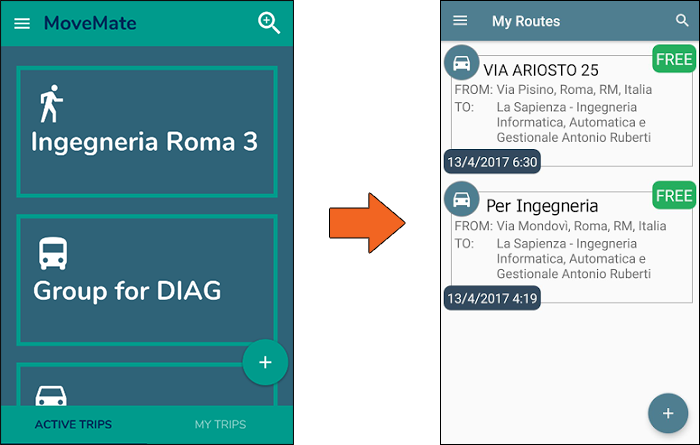
\includegraphics[width=1\textwidth]{path}
  \caption{Lista percorsi disponibili (prima e dopo)}
  \label{fig:path}
\bigskip
  \centering
    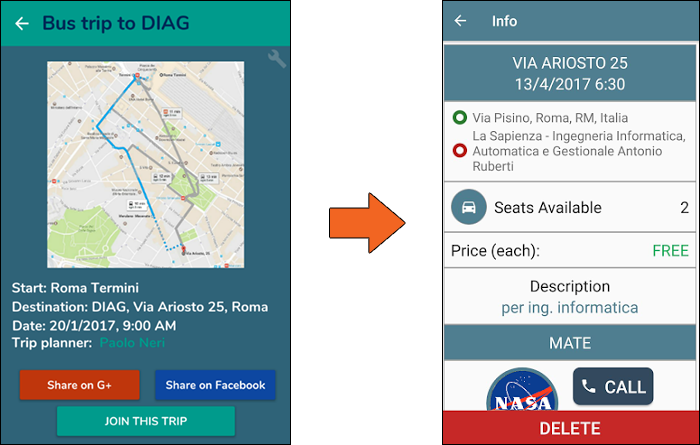
\includegraphics[width=1\textwidth]{path-info}
  \caption{Dettagli percorso (prima e dopo)}
  \label{fig:path-info}
\end{minipage}
\end{figure}
\FloatBarrier


\subsection{Librerie esterne}
Il lavoro necessario a completare tutte le funzioni dell'applicazione sarebbe diventato estenuante senza l'uso delle librerie, native e non.
Per implementare features preesistenti e per poter rendere il codice modulare e intuitivo sono state usate librerie provenienti prevalentemente dalla piattaforma GitHub\footnote{GitHub è un servizio di hosting per progetti software prevalentemente open-source. Il nome "GitHub" deriva dal fatto che GitHub è una implementazione dello strumento di controllo versione distribuito Git.}, piattaforma per la condivisione di progetti software, oltre a quelle proprietarie di Google. A tal fine, GitHub ha dato modo di esplorare sul campo il concetto di opensource che ha permesso di velocizzare e semplificare il lavoro, senza dover scrivere da zero porzioni di codice già esistenti. L’ecosistema Android, ben predisposto all’utilizzo di librerie esterne, ha garantito infine una rapida assimilazione del concetto di libreria fino a quel momento a me sconosciuto dal punto di vista pratico.
Le librerie usate spaziano dall’arricchimento della grafica per un migliore feedback da parte dell’utente, al download e compressione delle immagini per rendere l’applicazione e il carico verso il server leggeri, fino alla creazione dei percorsi sui quali si basa l'applicazione. Punto focale della descrizione di ogni percorso, infatti, è la mappa dello stesso.
Per integrarla nel progetto è stata usata la libreria Android-GoogleDirectionLibrary\footnote{\url{https://github.com/akexorcist/Android-GoogleDirectionLibrary}} che si occupa di creare il percorso, con il mezzo selezionato dall’utente, tramite chiamate REST verso i server Google.
Dati un punto di partenza e uno di arrivo, viene generato (onDirectionSuccess) un tracciato automatico sulla mappa che consente ai potenziali passeggeri di visualizzare l’ipotetico percorso che si effettuerà durante il viaggio.
La libreria sfrutta le API Google Maps che necessitano di una serverKey, generata nella Google API Console, per autenticare sviluppatore e applicazione e garantirne la proprietà.
\bigskip
\begin{minipage}{\linewidth}
\begin{lstlisting}[language=java, caption=Esempio integrazione Google API]
String serverKey = "AIzaSyDFWdlR5DG1VYXSaMwG62ilxxxxxxxxx";
LatLng origin = new LatLng(37.7849569, -122.4068855);
LatLng destination = new LatLng(37.7814432, -122.4460177);
String transitMode = TransportMode.DRIVING;
GoogleDirection.withServerKey(serverKey)
    .from(origin)
    .to(destination)
    .transitMode(transitMode)
    .execute(new DirectionCallback() {
        @Override
        public void onDirectionSuccess(Direction direction, String rawBody) {
            // successo 
        }

        @Override
        public void onDirectionFailure(Throwable t) {
            // gestione errore 
        }
    });
\end{lstlisting}
\end{minipage}
\FloatBarrier


\chapter{Conclusione}

\section{Considerazioni}
Questo progetto mi ha fatto entrare nel vivo del lavoro di programmazione e mi ha permesso di andare oltre lo studio astratto della tecnologia Android, mettendomi nella condizione di relazionarmi, dal punto di vista applicativo, con nuovi linguaggi quali ASP.Net per la gestione dei controller lato server. 
Il mio background accademico, nello specifico la conoscenza del paradigma REST, ha fornito la base astratta che mi ha permesso di giungere, nella sfera pratica, alla risoluzione di problemi in merito alla comunicazione tra l’applicazione ed il server. 
Nello sviluppo dell’applicazione sono stati coinvolti anche gli utenti finali tramite sondaggi relativi all’ UI/UX lungo tutto il periodo di sviluppo: sulla base dei dati emersi è stato fatto sì che venissero presi quegli accorgimenti che, mettendo a proprio agio l’utente, rendono un’applicazione una buona applicazione.
Per una migliore "esperienza utente" (User eXperience - UX) siamo partiti dalle caratteristiche di altri servizi di carsharing e ridesharing presenti sul mercato per poi adattarli e renderli conformi ai gusti, alle esigenze e alle preferenze di un pubblico giovane.
La realizzazione del progetto è avvenuta nei tempi previsti. Ciò è stato reso possibile anche grazie all'aiuto dei tutor che hanno saputo guidarci nello sviluppo grazie alle loro competenze e conoscenze acquisite sul campo, ma soprattutto al lavoro di squadra. La collaborazione con i tutor e la sintonia e la serietà che si è venuta a creare nel gruppo hanno fatto sì che il lavoro finale risultasse completo e curato. 
Le nostre conoscenze tecniche acquisite prima e durante il progetto sommate all’affiatamento venutosi a creare nel gruppo hanno reso questo workshop una bellissima esperienza che, tornando indietro, rifarei molto volentieri.
Al termine del percorso sono stati raggiunti gli obiettivi prefissati, sono state acquisite le competenze ed abilità di base per lo sviluppo di un’applicazione, dalla sua fase embrionale di idea al rilascio al pubblico con relativi feedback positivi da parte dell’utenza. 
Si è imparato a lavorare in gruppo condividendo idee, ma soprattutto aiutandosi a vicenda per raggiungere un obbiettivo comune e superare le difficoltà.

\section{Progetto finale}
Tutto il codice su cui si è lavorato durante i tre mesi di progetto sono stati catalogati sulla piattaforma GitHub e il progetto completo è visualizzabile nella relativa repository.
\begin{itemize}
\item \textbf{Codice sorgente client:} \url{https://github.com/movers-gcw/movemate_android}
\item \textbf{Codice sorgente server ASP.Net:} \url{https://github.com/movers-gcw/movemate_api}
\item \textbf{Sito web progetto:} \url{https://movers-gcw.github.io}
\end{itemize}


\end{document}